\chapter{Landmark Graph Construction}
\begin{defn}[\emph{Landmark}]\label{Def:ldmk}
A landmark is a road segment that is frequently traversed by taxi drivers based on the taxi GPS trajectory database. \cite{TDR10}
\end{defn}
The concept of a landmark is proposed primarily for two reasons. First, as mentioned in the Section~\ref{Sec:limitation}, the taxi GPS trajectories do not necessarily cover every road segment in a city's road network and the low-sampling-rate problem makes determining the exact route that a taxi has traversed difficult. Therefore, it is not possible to estimate the time cost for each road segment. However, ignoring the length of a road segment and considering it as an abstract ``landmark'' make estimating the travel time between two \emph{landmarks} easy. 

Moreover, the notion of a landmark closely follows the way how drivers remember the driving routes in daily life\cite{TDR10}. For instance, a driving route could be described as ``go straight on the 4th Avenue, turn right at the 7th Street and exit at the Smith Road''. Drivers tend to use familiar road segments as landmarks to guide their directions.

This chapter describes the procedures for constructing a landmark graph in order to estimate the time cost between two landmarks. But before that, the taxi GPS trajectories must be separated into a set of \emph{trip}s.

\section{Trip Identification}
\begin{defn}[\emph{Trip}]\label{Def:trip}
A trip is a set of chronologically ordered GPS records belonging to one taxi that satisfies either condition:
\begin{enumerate}
\item A passenger is on the taxi, namely, the OCCUPIED field has a value of 1 for all the GPS records or, 
\item No passenger is on the taxi, but the time difference between \emph{any} two consecutive GPS records is less than 3 minutes.
\end{enumerate}
\end{defn}

\begin{table}
\centering
\begin{tabular}{ | l | l | l | }
\hline
\textbf{Field} & \textbf{Explanation} \\ \hline
DataUnitID & Nominal primary key for each record \\ \hline
BD09\_LONG & Longitude encoded in BD-09 format\\ \hline
BD09\_LAT & Latitude encoded in BD-09 format\\ \hline
STREET & Street name\\ \hline
\end{tabular}
\caption{Additional fields added to data set}\label{Ta:addtional_field}
\end{table}

%\csvreader
%[tabular= | l | l | l | l | l | l | l | l | l | l | l | l | l |
%    table head=\hline & DataUnitID & CUID & UTC & UnixEpoch & GPS_LONG & GPS_LAT & BD09_LONG & BD09_LAT & Street & Head & Speed & Occupied & TripID\\\hline,
%    late after line=\\\hline]%
%{tripsample.csv}{DataUnitID=\DataUnitID, CUID & UTC & UnixEpoch & GPS_LONG & GPS_LAT & BD09_LONG & BD09_LAT & Street & Head & Speed & Occupied & TripID}%
%{\thecsvrow & \surname~\name & \age}%

%\csvreader[tabular=| l | l | l |,
%    table head=\hline & Name & Age\\\hline,
%    late after line=\\\hline]%
%{scientists.csv}{name=\name,surname=\surname,age=\age}%
%{\thecsvrow & \surname~\name & \age}%

The original data set came in a binary file format. After the data set was decoded and imported into a MySQL database, the first step in data cleaning was \textbf{to delete all records with zero value in the SPEED field}, since when a taxi is stationary it yields no valuable information about the \emph{trajectory} it is moving along. While being stationary could be due to a traffic jam, this kind of information is well captured by the time difference between the last \emph{non-stationary} data point and the next \emph{non-stationary} data point. 

In addition, all records must have a \emph{unique} pair of CUID and UNIX\_EPOCH fields, since it is not possible for a taxi to appear in two different locations at the same moment in time. This kind of error is likely due to some errors in aggregating the original data set.

\section{Reverse Geocoding}
After the data set was cleaned, the next step was to map each GPS data point to a road segment, which is also known as \emph{reverse geocoding}. A number of algorithms\cite{MAP09} have been proposed for this purpose, but most of them require an additional GIS\footnote{Geographic Information System} database of the road network in Beijing. This project adopted an alternative strategy which leveraged on the existing public APIs\footnote{Application Programming Interface} for reverse geocoding. 

Currently, a number of online mapping platforms provide reverse geocoding services as part of their developer APIs. Amongst others, Google Maps and Baidu Maps offer relatively stable and fast reverse geocoding services. However, due to the ``China GPS shift problem''\cite{GSHF17} where coordinates encoded in WGS-84 format are required by regulations to be shifted by a large and variable amount when displayed on a street map, Google Maps is not able to display a GPS data point correctly because it only supports WGS-84 formats. Figure~\ref{Fig:gps_shift} illustrates the effect of such shift, with the correct location displayed on the right. 

\begin{figure}[h]
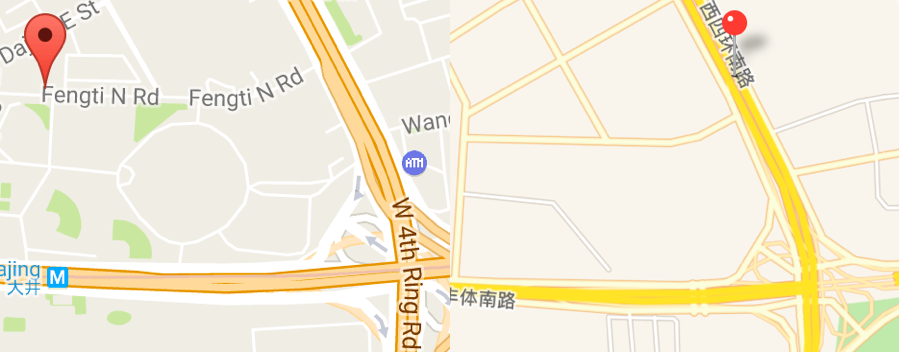
\includegraphics{gps_shift}
\centering
\caption{China GPS shift problem}\label{Fig:gps_shift}
\end{figure}

Baidu Maps, on the other hand, has been using their own coordinate system, BD-09, which is an improved version of the Chinese official coordinate system, GCJ-02. Baidu provides a set of APIs to convert WGS-84 coordinates into BD-09 ones. Therefore, to reverse-geocode the data points, the coordinates must be converted to BD-09 format. To store the converted coordinates as well as the street names obtained from reverse geocoding, four new fields were added to the original data set as shown in Table~\ref{Ta:addtional_field}.

\begin{table}
\centering
\begin{tabular}{ | l | l | l | }
\hline
\textbf{Field} & \textbf{Explanation} \\ \hline
DataUnitID & Nominal primary key for each record \\ \hline
BD09\_LONG & Longitude encoded in BD-09 format\\ \hline
BD09\_LAT & Latitude encoded in BD-09 format\\ \hline
STREET & Street name\\ \hline
\end{tabular}
\caption{Additional fields added to data set}\label{Ta:addtional_field}
\end{table}

In order to use Baidu APIs for coordinate conversion, the following system architecture was set up as shown in Figure~\ref{Fig:basic_architecture}. The Apache HTTP server hides the MySQL database and sends HTTP POST request to Baidu Maps Web API to get converted coordinates. Then it updates the database through PHP \emph{mysqli} utilitity. 

\begin{figure}[h]
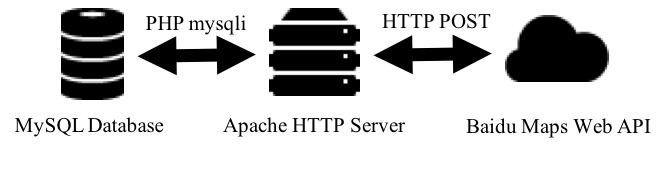
\includegraphics{basic_architecture}
\centering
\caption{Basic system architecture}\label{Fig:basic_architecture}
\end{figure}

After the coordinates were converted from WGS-84 format to BD-09 format, Baidu Maps Web API was used to reverse geocode all GPS data points. However, the system architecture was slightly changed, to accommodate the change in technology used. For reverse geocoding, AJAX\footnote{Asynchronous JavaScript and XML} was used to communicate with the Baidu Maps Web API for speed and unlimited number of requests per day. Therefore, one additional layer was added to the existing system architecture as shown in Figure~\ref{Fig:ajax_architecture}. 

\begin{figure}[h]
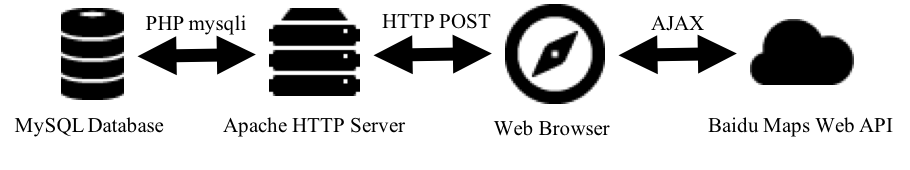
\includegraphics{ajax_architecture}
\centering
\caption{Augmented system architecture}\label{Fig:ajax_architecture}
\end{figure}

Executed in a web browser environment, AJAX sent HTTP POST requests to the Apache HTTP server to fetch the converted coordinates in BD-09 format which were subsequently sent to the Baidu Maps Web API server \emph{asynchronously} via HTTP GET requests. Once the server responded with the name of the road segment, AJAX updated the database by sending another HTTP POST request to the Apache HTTP server. The asynchronous nature of this architecture, however, caused a few problems which are addressed in Section~\ref{outlier_detecting}. 

\section{Outlier Detection}\label{outlier_detecting}
\subsection{Motivation for Outlier Detection}
The Baidu Maps Web API for reverse geocoding is stable and fast, but does not produce no errors. Sometimes, a GPS data point may be mapped to a main road but actually it is on the side road, which is one of the limitations mentioned in Section~\ref{Sec:limitation} or it is actually mapped to a street that Baidu Maps does not recognise. In neither case will Baidu Maps produce a correct reverse geocoding. Moreover, the reverse geocoding process is asynchronous, which means that it is being performed in the background in parallel with the main application thread. Therefore, it is inevitable that some street names may get lost when the records are being updated or a record is updated with a wrong street name. Figure~\ref{Fig:exmp_outlier} shows a drastic example.

\begin{figure}[h]
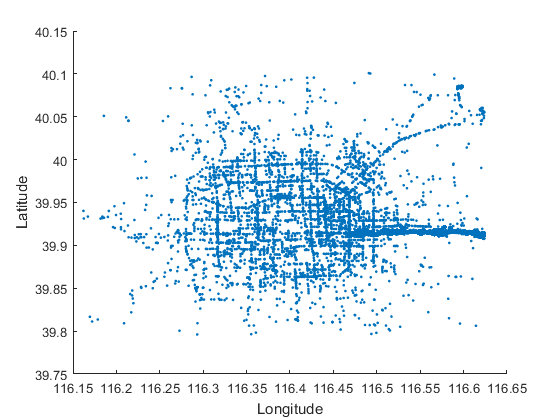
\includegraphics{long_lat_plot}
\centering
\caption{Example of outliers}\label{Fig:exmp_outlier}
\end{figure}

In this example, the Baidu Maps believes that all data points plotted belong to a particular street. But when plotted on a 2-D plane, these data points almost represent the \emph{entire} road network in Beijing. The actual, correct street is represented in the figure as the \emph{thickest} line on the right half of the figure with a longitude ranging from 116.45\textdegree~to 116.65\textdegree.~Erroneous records like those not on the thickest line are known as \emph{outliers} and must be properly identified and removed. This project proposes a novel outlier detection approach based on unsupervised learning whose principle behind is based on Theorem~\ref{Theorem: majority_clustering}.

\begin{defn}[\emph{Reasonable reverse geocoder}]\label{Def:reasonable_geocoder}
A reasonable reverse geocoder always gives its best matching from a GPS data point to a street whenever possible and has an accuracy more than 50\%.
\end{defn}

\begin{theorem}[\emph{Majority Clustering Theorem}]\label{Theorem: majority_clustering}
If a \emph{reasonable reverse geocoder} is used to reverse geocode a set of GPS data points which are mapped to a particular street \emph{in reality}, then, when plotted on a 2-D plane, majority (more than 50\%) of the points must be clustered together to form a rough shape that is similar to the shape of the street that they are supposed to be mapped to. 
\end{theorem}

\begin{proof}
Proof by contradiction. Assume, for the purpose of contradiction, majority (more than 50\%) of the data points that are \emph{indeed} located on the same street are scattered arbitrarily on a 2-D plane after being reverse-geocoded by a reasonable reverse geocoder. In particular, when plotted on a 2-D plane, majority of them do not form a similar shape to that of the street they are supposed to be mapped to. Then, the majority must have been erroneously mapped to some other streets because no single street covers the whole city area. Thus, the reasonable reverse geocoder has only achieved an accuracy less 50\%, which contradicts the Definition~\ref{Def:reasonable_geocoder} of a reasonable reverse geocoder. 
\end{proof}

\subsection{Outlier Identification}
Apparently, Baidu Maps provides a reasonable reverse geocoder because it is of industrial-grade quality and has an accuracy larger than 50\%. Therefore, if a set of points belong to a particular street, after reverse-geocoded by Baidu Maps, majority of them should be clustered to assume a rough shape of that street according to Theorem~\ref{Theorem: majority_clustering}. Based on that, an unsupervised learning technique --- clustering can be used to separate the correctly mapped data points from outliers. 

Many clustering techniques are available\cite{LO05}. Since each record can be represented graphically by a point on a 2-D plane with longitute as the $x$ axis and latitude as the $y$ axis, a \textbf{self-organising feature map}\cite{TK82}(SOFM) seems to be an appropriate technique to use. 

\begin{figure}[h]
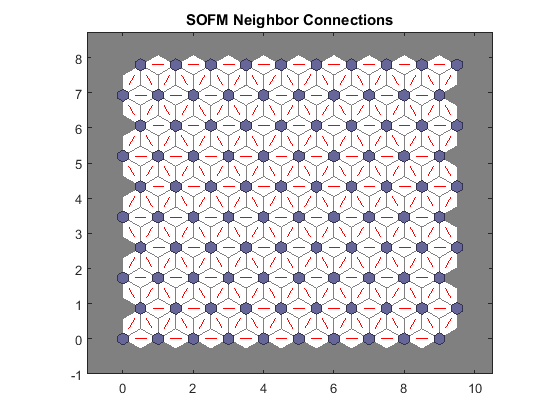
\includegraphics{neighbour_connections}
\centering
\caption{An example of SOFM}\label{Fig:neighbour_connections}
\end{figure}

A self-organising feature map is a form of artificial neural network. It consists of a pre-defined number of interconnected neurons distributed over a 2-D plane as shown in Figure~\ref{Fig:neighbour_connections}. Prior to training, the neurons are randomly scattered among the data points and gradually move to the centroids of the data clusters they represent as they learn the \emph{features} of the training data. Upon termination of the training, all data points near to a particular neuron, in terms of Euclidean distance\footnote{Other distance measures are also possible.}, are assigned to the cluster that neuron represents. Figure~\ref{Fig:sofm_weights} shows the results after the clustering is completed. 

\begin{figure}[h]
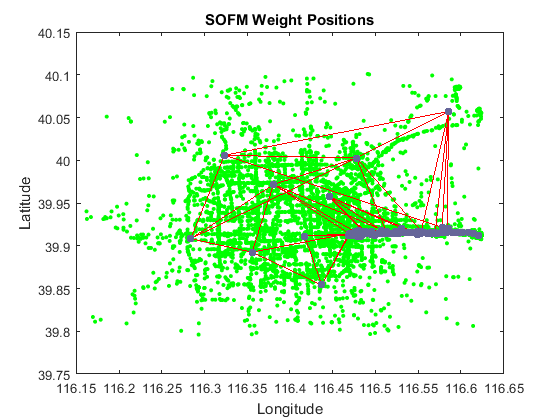
\includegraphics{sofm_weights}
\centering
\caption{Neuron positions after training}\label{Fig:sofm_weights}
\end{figure}

It is clear from the figure that while some neurons represent the clusters of outliers, majority of the neurons are clustered to \emph{cover} the correct street they should represent. A $10\times10$ SOFM was used in this project, so there were at most 100 neurons or equivalently, 100 clusters. Each cluster had a different size. To ensure a thorough removal of the outliers, \textbf{only the top 50\% largest clusters were considered as clusters of correct data points which are called ``legal clusters''. All other clusters were deemed as clusters of outliers}. 

\subsection{Outlier Removal}
Once the legal clusters were identified, a distance threshold was set to remove outliers so that \textbf{whenever the minimum distance between a data point and all centroids of the legal clusters was above the threshold, that data point would be considered as an outlier and removed}. The python-like pseudocode in Listing~\ref{List:code_outlier} describes this idea with more clarity.

%\begin{minipage}{\linewidth}
\begin{lstlisting}[language = Python, caption = {Pseudocode for outlier detection}, label = {List:code_outlier} ,frame=single, numbers=left,stepnumber=1]
for record in records:
	min_distance = math.inf // infinity
	for centroid in centroids:
		min_distance = min(min_distance, \
			get_distance(record, centroid))
	if min_distance > threshold:
		remove(records, record)
\end{lstlisting}
%\end{minipage}

However, the \emph{distance} between a data point and a centroid is not as straightforward as Euclidean distance. A centroid, to some extent, can be imagined as a \emph{real} point on the Earth's surface. To calculate the distance between a data point and a centroid is to calculate the spherical distance which is given by the haversine formula in Theorem~\ref{Theorem: haversine}. 

\begin{theorem}[\emph{Haversine Formula}]\label{Theorem: haversine}
Given two points $P(\lambda_1,\varphi_1)$ and $Q(\lambda_2,\varphi_2)$ on the surface of a sphere, where $\lambda$ and $\varphi$ represent longitude and latitude in radians, their spherical distance (the distance along a great circle of the sphere) is given by\cite{FI06}
\begin{equation}
d = 2R\arcsin{\sqrt{\sin^2\frac{\varphi_2 - \varphi_1}{2} + \cos\varphi_1\cos\varphi_2\sin^2\frac{\lambda_2 - \lambda_1}{2}}} 
\end{equation}
where $R$ is the radius of the sphere. 
\end{theorem}

Since the Earth is not a perfect sphere, $R$ varies with latitude. Theorem~\ref{Theorem: radius_latitide} suggests how to calculate the Earth radius at any latitude. 

\begin{theorem}[\emph{Radius at any Latitude}]\label{Theorem: radius_latitide}
Given a latitude $\varphi$ in radians, a polar radius $R_{p}$ and an equatorial radius $R_{e}$, the spheroid's radius at that latitude is given by\cite{EAR17}
\begin{equation}
R(\varphi) = \sqrt{\frac{(R_{e}^2\cos\varphi)^2 + (R_{p}^2\sin\varphi)^2}{(R_{e}\cos\varphi)^2 + (R_{p}\sin\varphi)^2}}
\end{equation}
\end{theorem}

It is known that $R_{e} = 6,378,137$ metres and $R_{p} = 6,356,752$ metres on the Earth\cite{NASA16} and that Beijing's latitude is about 39\textdegree N. Therefore, the distance between a data point and a centroid can be calculated. For this project, two thresholds were selected: 30 metres and 50 metres. The thresholds were set in a way that it ensured there was sufficient data for subsequent machine learning tasks while the estimates were as least affected as possible by outliers. If the threshold were set to a too small value, the remaining data could not have been sufficient; on the other hand, however, if the threshold were set to a too big value, the accuracy of the final results would have been subject to outliers. 

\begin{figure}[h]
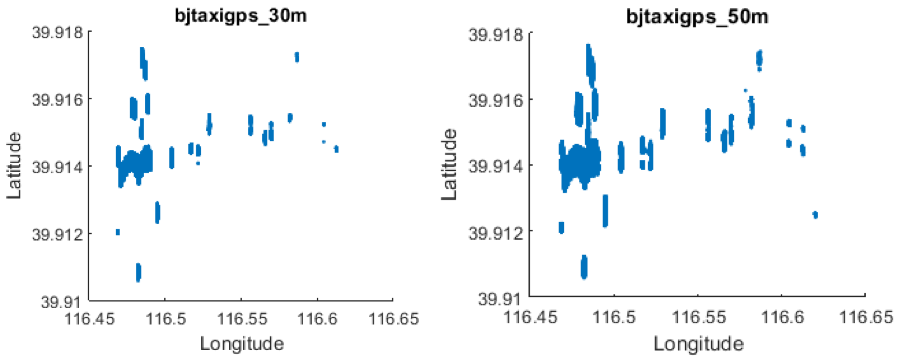
\includegraphics{30m_50m}
\centering
\caption{Plot of data points after outlier removal}\label{Fig:after_removal}
\end{figure}

After the outliers were removed, two data sets remained. They are hereinafter referred to as \emph{bjtaxigps\_30m}, where outliers were filtered by a threshold of 30 metres and \emph{bjtaxigps\_50m}, where outliers were filtered by a threshold of 50 metres, respectively. bjtaxigps\_30m contains approximately 51 million records while bjtaxigps\_50m has 59 million. All algorithms described hereinafter are applicable to both data sets. Figure~\ref{Fig:after_removal} gives a plot of the data points from both data sets. Clearly, the data points are now contained in a much smaller area and roughly form a shape similar to that of the street they are mapped to. 